\documentclass{beamer}
\usepackage[orientation=landscape,size=custom,width=16,height=9,scale=0.5,debug]{beamerposter}

%% FONT
\usepackage[default]{comfortaa}
\usepackage[T1]{fontenc}

%% BIB
\usepackage[style=authoryear,backend=biber,url=false]{biblatex}
\addbibresource{nems.bib}

%% FIGURES
\usepackage[export]{adjustbox}
%\usepackage{epstopdf}
\graphicspath{{figures/}}
\DeclareGraphicsExtensions{.pdf,.jpg}

%% FONTS
\usepackage{amsfonts,amssymb,amsmath}

%% COLORS
%\definecolor{StrongBlue}{HTML}{043C6B}
%\definecolor{SoftBlue}{HTML}{3F8FD2}
%\definecolor{StrongGreen}{HTML}{00733E}
%\definecolor{SoftGreen}{HTML}{36D88E}
%\definecolor{StrongRed}{HTML}{A64B00}
%\definecolor{SoftRed}{HTML}{FF9640}

%% RM NAV SYMBOLS
\setbeamertemplate{navigation symbols}{}

%% Content begins %%

\title{Nested Effects Models and extensions}
\subtitle{group meeting}
\date{July 15, 2016}
\author{Yuriy Sverchkov}
\institute{University of Wisconsin--Madison}

\begin{document}
\begin{frame}[plain]
  \titlepage
\end{frame}

\begin{frame}[plain]
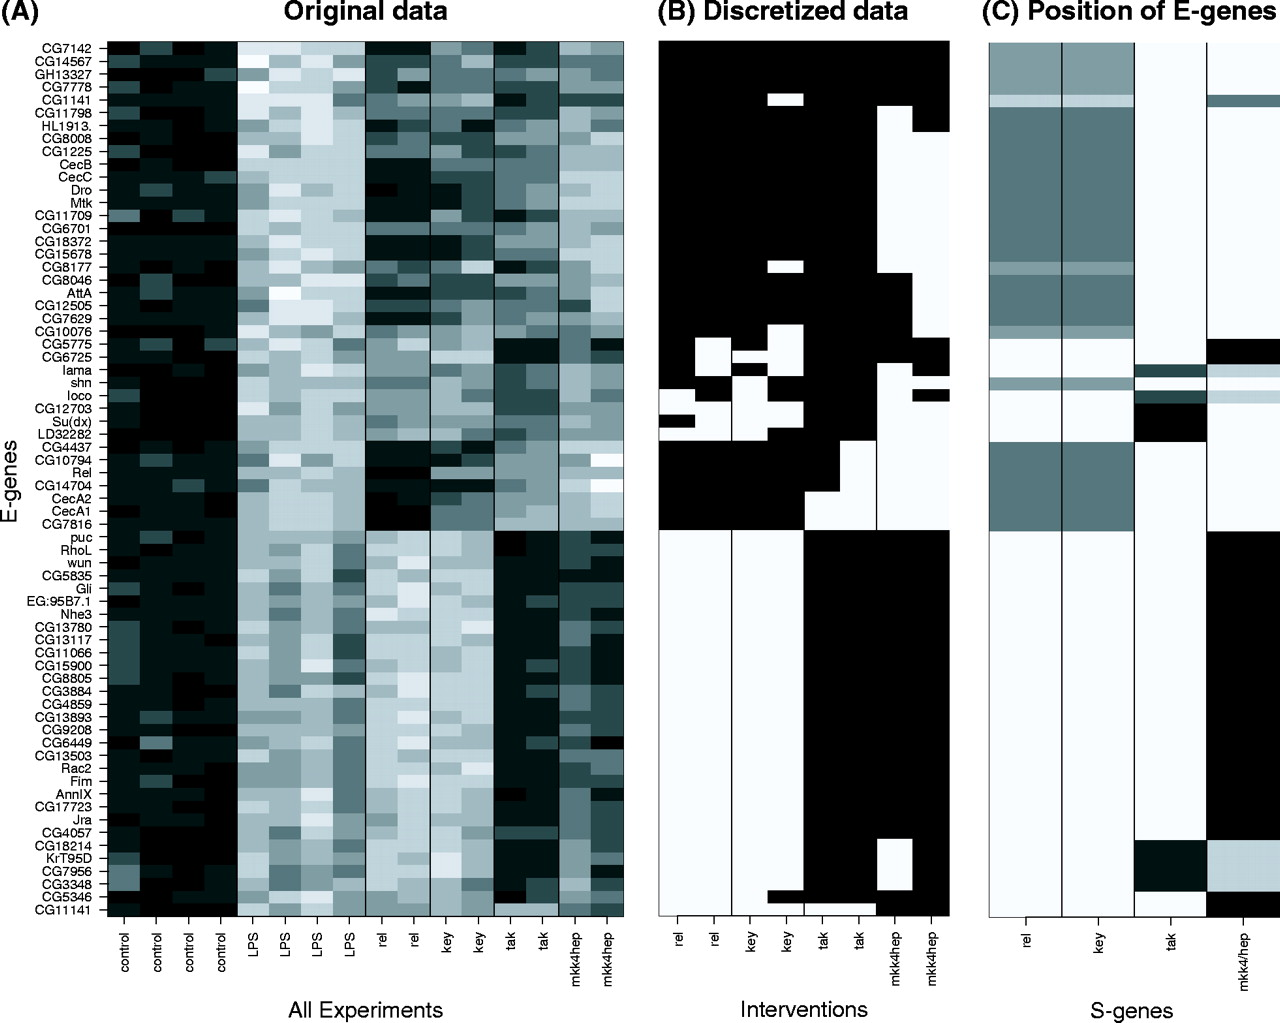
\includegraphics[valign=c,height=4cm,trim={0 0 22cm 0}, clip]{F3_large.jpg}
\hfill {\Huge $\rightarrow$} \hfill
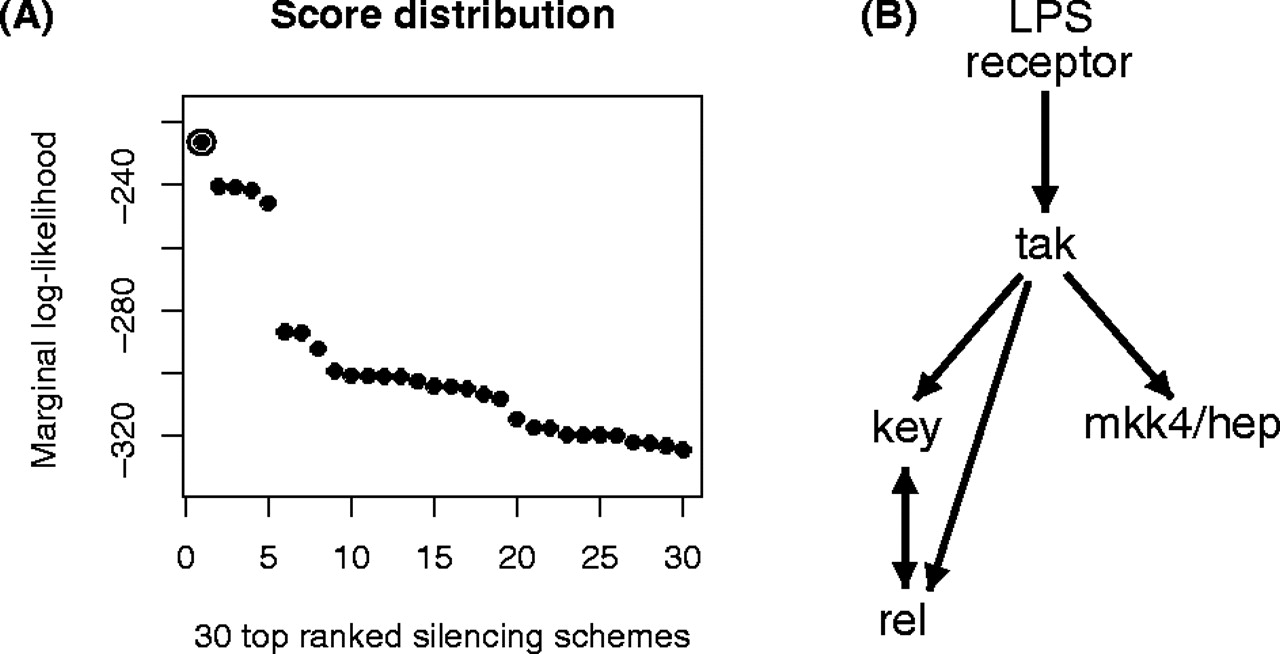
\includegraphics[valign=c,height=2cm,trim={30cm 0 0 0}, clip]{F4_large.jpg}

\raggedleft \scriptsize \cite{Markowetz01012005}
\end{frame}

\begin{frame}{Nested Effects Models (NEM)}
\begin{columns}
\column{0.4\textwidth}
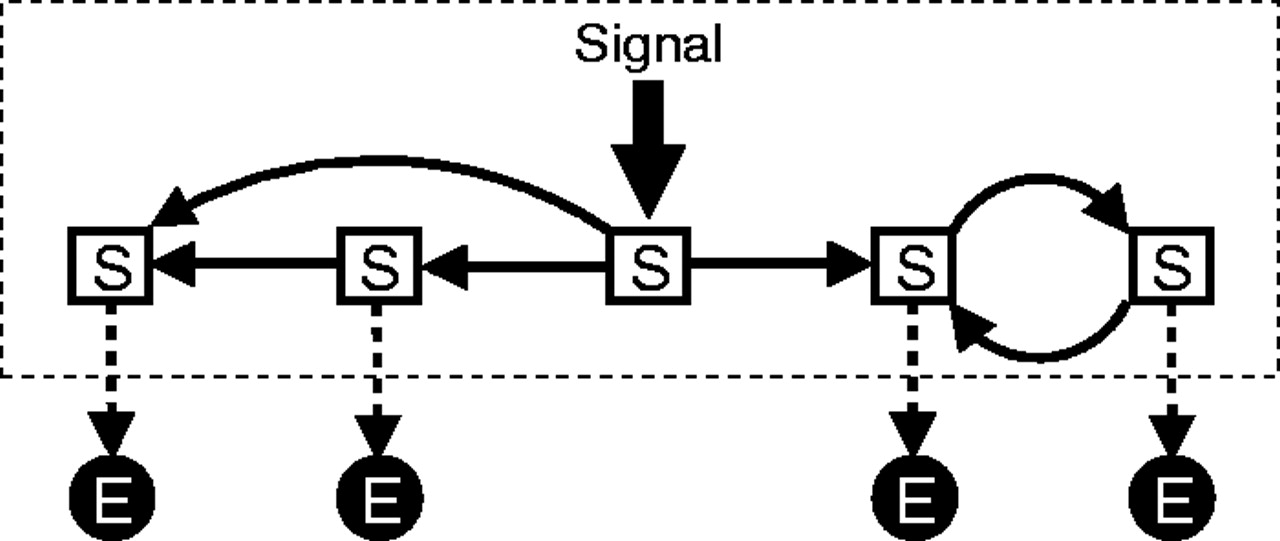
\includegraphics[width=0.9\textwidth]{F1_large.jpg}

\column{0.5\textwidth}
\begin{itemize}
  \item[S-genes] are the knockout genes
  \item[E-genes] are the measured genes
\end{itemize}
\end{columns}
\pause
\begin{itemize}
  \item \textbf{Main principle:} If an \textbf{E-gene} is differentially expressed subject to a knockout of an \textbf{S-gene}, they need to connect
  \item \textbf{Modeling constraint:} An \textbf{E-gene} can only have a direct connection to only one \textbf{S-gene}
\end{itemize}
\end{frame}

\begin{frame}{The model induces a \textbf{nesting} of E-gene sets}
\centering
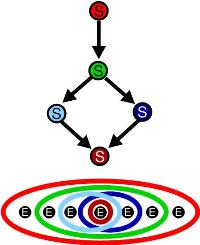
\includegraphics{NestedEffects.jpg}
\end{frame}

\begin{frame}{Formulated as likelihood maximization}
\[ P( D | \Phi ) = \frac{ 1 }{ n^m } \prod_{i=1}^m \sum_{j=1}^n \prod_{k=1}^l P( e_{ik} | \Phi, \theta_i = j ) \]

\[ P( e_{ik} | \Phi, \theta_i = j ) = \left\{
  \begin{array}{ccl}
    e_{ik} = 1 & e_{ik} = 0 \\
    \alpha & 1-\alpha &\text{if } \Phi \text{ predicts no effect} \\
    1-\beta & \beta &\text{if } \Phi \text{ predicts effect}
  \end{array}
 \right.
\]

\scriptsize
\begin{columns}
\column{0.3\textwidth}
$i = 1,\ldots,m$ - E-genes \\
$j = 1,\ldots,n$ - S-genes \\
$k = 1, \ldots, l$ - replicates
\column{0.3\textwidth}
$\Phi$ - network structure \\
$\theta_i$ - E-gene attachments \\
$e_{ik}$ - effect $i$ in experiment $k$ \\
\column{0.3\textwidth}
$\alpha$ - type-I error \\
$\beta$ - type-II error \\
\end{columns}

\vfill

\fullcite{Markowetz01012005}

\end{frame}

\begin{frame}{Extensions and improvements}
\begin{description}
 \item[\cite{Markowetz01012005}] - original paper
 \item[\cite{markowetz2007nested}] - scalable structure learning by aggregating three-node graphs
 \item[\cite{frohlich2007large}] - use of continuous input data, structure search by MCMC, modularization for structure search
 \item[\cite{vaske2009factor}] - inference using factor graphs
 \item[\cite{anchang2009modeling}] - extension to time-series data
\end{description}
\end{frame}

\begin{frame}{Context-specific nested effects models (CSNEMs)}
\begin{columns}
\column{0.5\textwidth}
NEM
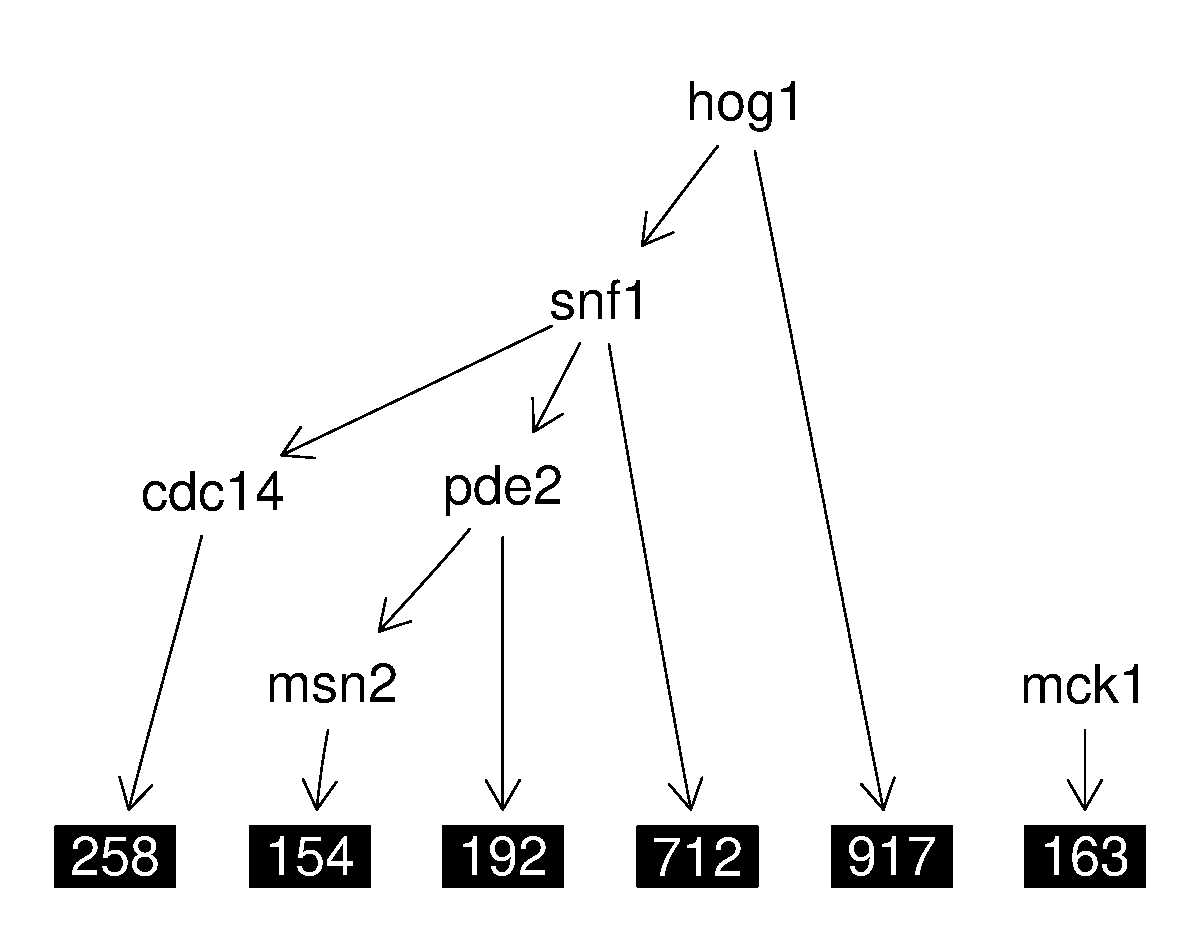
\includegraphics[width=\textwidth]{nem}
\column{0.5\textwidth}
CSNEM
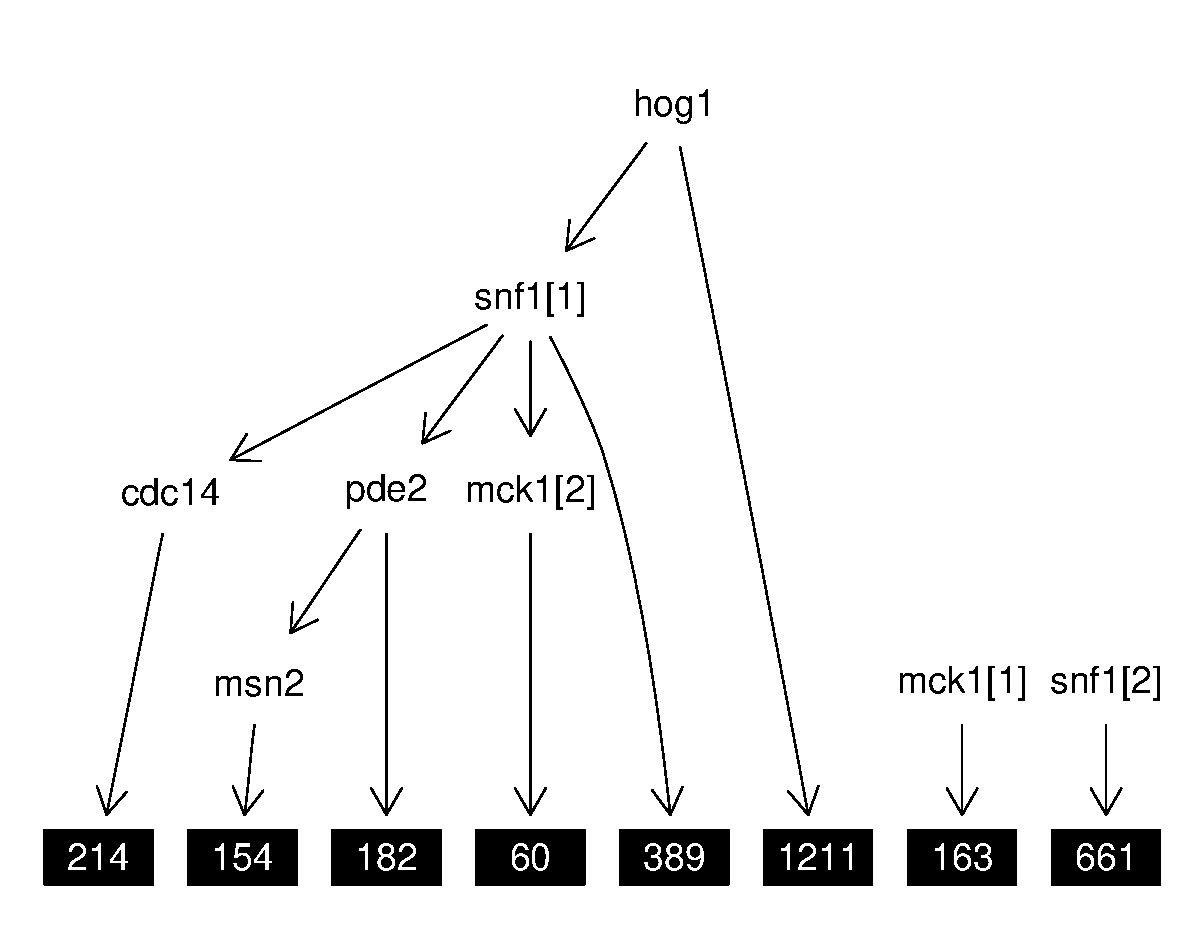
\includegraphics[width=\textwidth]{csnem}
\end{columns}
\end{frame}

\begin{frame}{Learning a 2-CSNEM model greedily}
\begin{itemize}
 \item Split E-genes into 2 groups randomly
 \item Repeat:
 \begin{itemize}\normalsize
  \item Learn NEM for each group
  \item Find the worst-fitting E-gene and move it to the other group
  \item Repeat until NEM likelihood scores stop improving
 \end{itemize}
 \item Compare learned NEMs; for each S-gene that has different ancestors, create a duplicate, and move the E-gene effects for it in one group to the duplicate
 \item Learn NEM from new profile with extended S-gene set
\end{itemize}
\end{frame}

\end{document}